\section{Projektplanung}
\label{sec:chapterexample}

\subsection{Prozess}
\label{sec:chapterexample}

Als Entwicklungsprozess wird ein hybrides Vorgehensmodell eingesetzt welcher in Abbildung \ref{fig:hybridesModell} zu sehen ist. Im Rahmen einer Bachelor Arbeit, in der die Anforderungen und Analysen schon im Vorhinein im Fachmodul definiert worden sind, eignet sich am bestens ein lineares V-Modell. Ein solcher Prozess ist sehr schlank, übersichtlich und geeignet für die Grösse des Projekts.
\\
Was das V-Modell nicht erlaubt, ist eine ständige Iteration mit dem Kunden während der Entwurf/Implementierungsphase. Daraus ergibt sich, wie im Abbild unten gezeigt, ein hybrides Modell welches uns erlaubt, trotz der klar definierten Anforderungen, während der Entwurf- und der Implementierungsphase ein agiles Vorgehen mit der Kunde durchzuführen.
\\
Die im Fachmodul geleistete Arbeit gehört zu den ersten zwei Phasen des Modells. Wie im linearen Vorgehensmodell vorgegeben, beginnt die nächste Phase der Arbeit sobald die vorherige Phase abgeschlossen ist. Die ganze Bachelorarbeit basiert auf Evaluationen/Entscheidungen die in den ersten Phasen getroffen worden sind.  

\begin{figure}[htb!]
	\begin{center}
		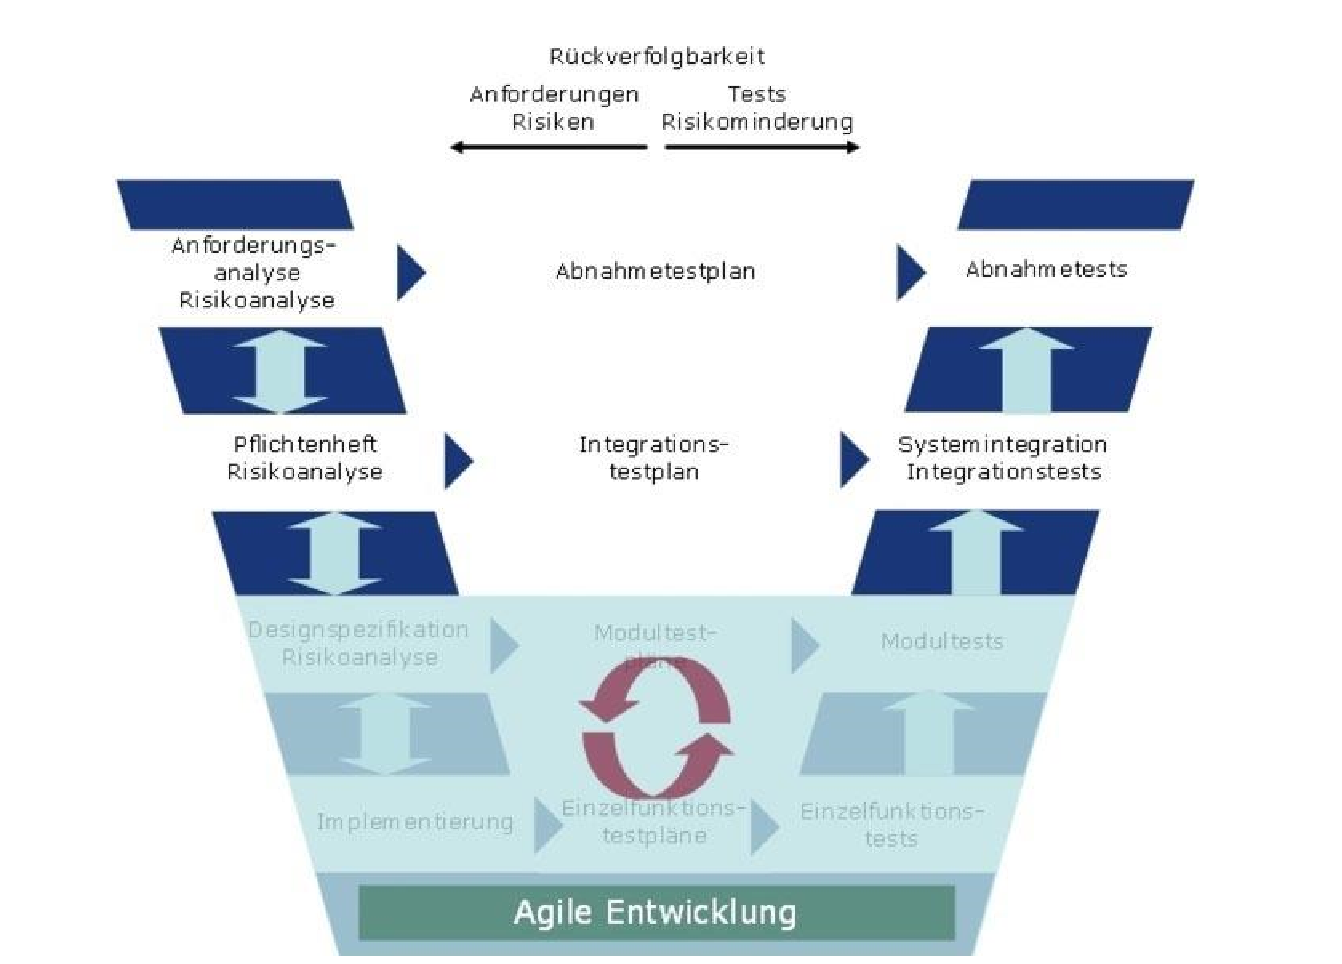
\includegraphics[width=0.89\textwidth]{hybridesModell}
		\caption[Hybrides Vorgehensmodell]{Hybrides Vorgehensmodell}
		\label{fig:hybridesModell}
	\end{center}
\end{figure}


\subsection{Zeitplanung}
\label{sec:zeitplanung}

Die folgenden Abbildungen stellen die Projektplanung und die Meilensteine zeitlich dar (\seeref{fig:projektPlanungAchse} \& \cref{fig:projektPlanung}). In die erste Woche werden die Hardware Komponenten, die mittlerweile schon bestellt wurden, getestet und zusammengebaut.
\\
Die nächste zwei Meilensteine sind Software-Ready Meilensteine. Die Software Programmierung wurde in zwei Teile geteilt.
\\ 
Bei Part 1 geht es um die Skripts die Serverseitig kleine Aufgaben übernehmen. Part 2 ist der grösste Programmierung teil. Da werden die Webapplikationen entwickelt, die auf die Aussensprechstellen und auf die Mobile Geräte der Bewohner ausgeführt werden sollen.
\\
Die letzte Phase ist für die Optimierung und Reserve gedacht.

\begin{figure}[htb!]
	\begin{center}
		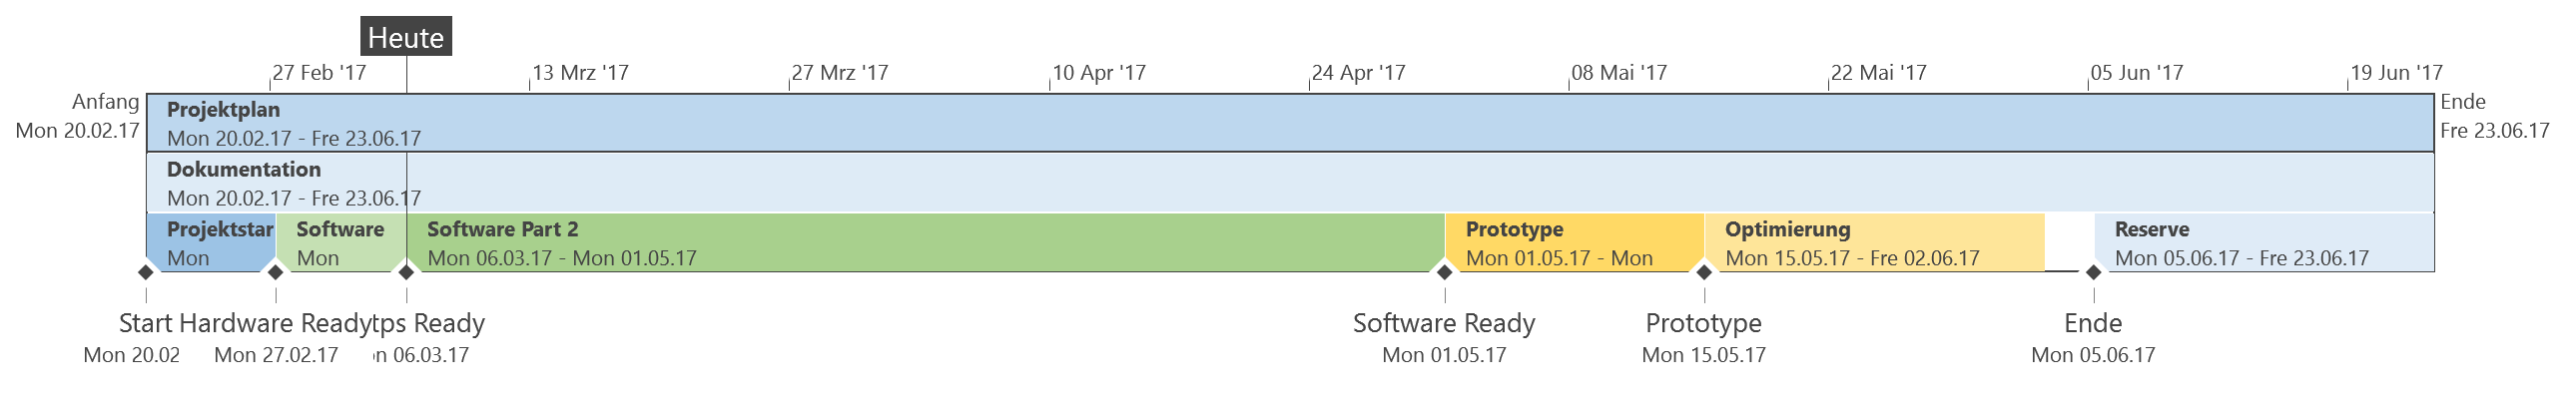
\includegraphics[width=1\textwidth]{projektPlanAchse}
		\caption[Projektplanung Meilensteine]{Zeitplanung mit Meilensteine}
		\label{fig:projektPlanungAchse}
	\end{center}
\end{figure}


\begin{figure}[htb!]
	\begin{center}
		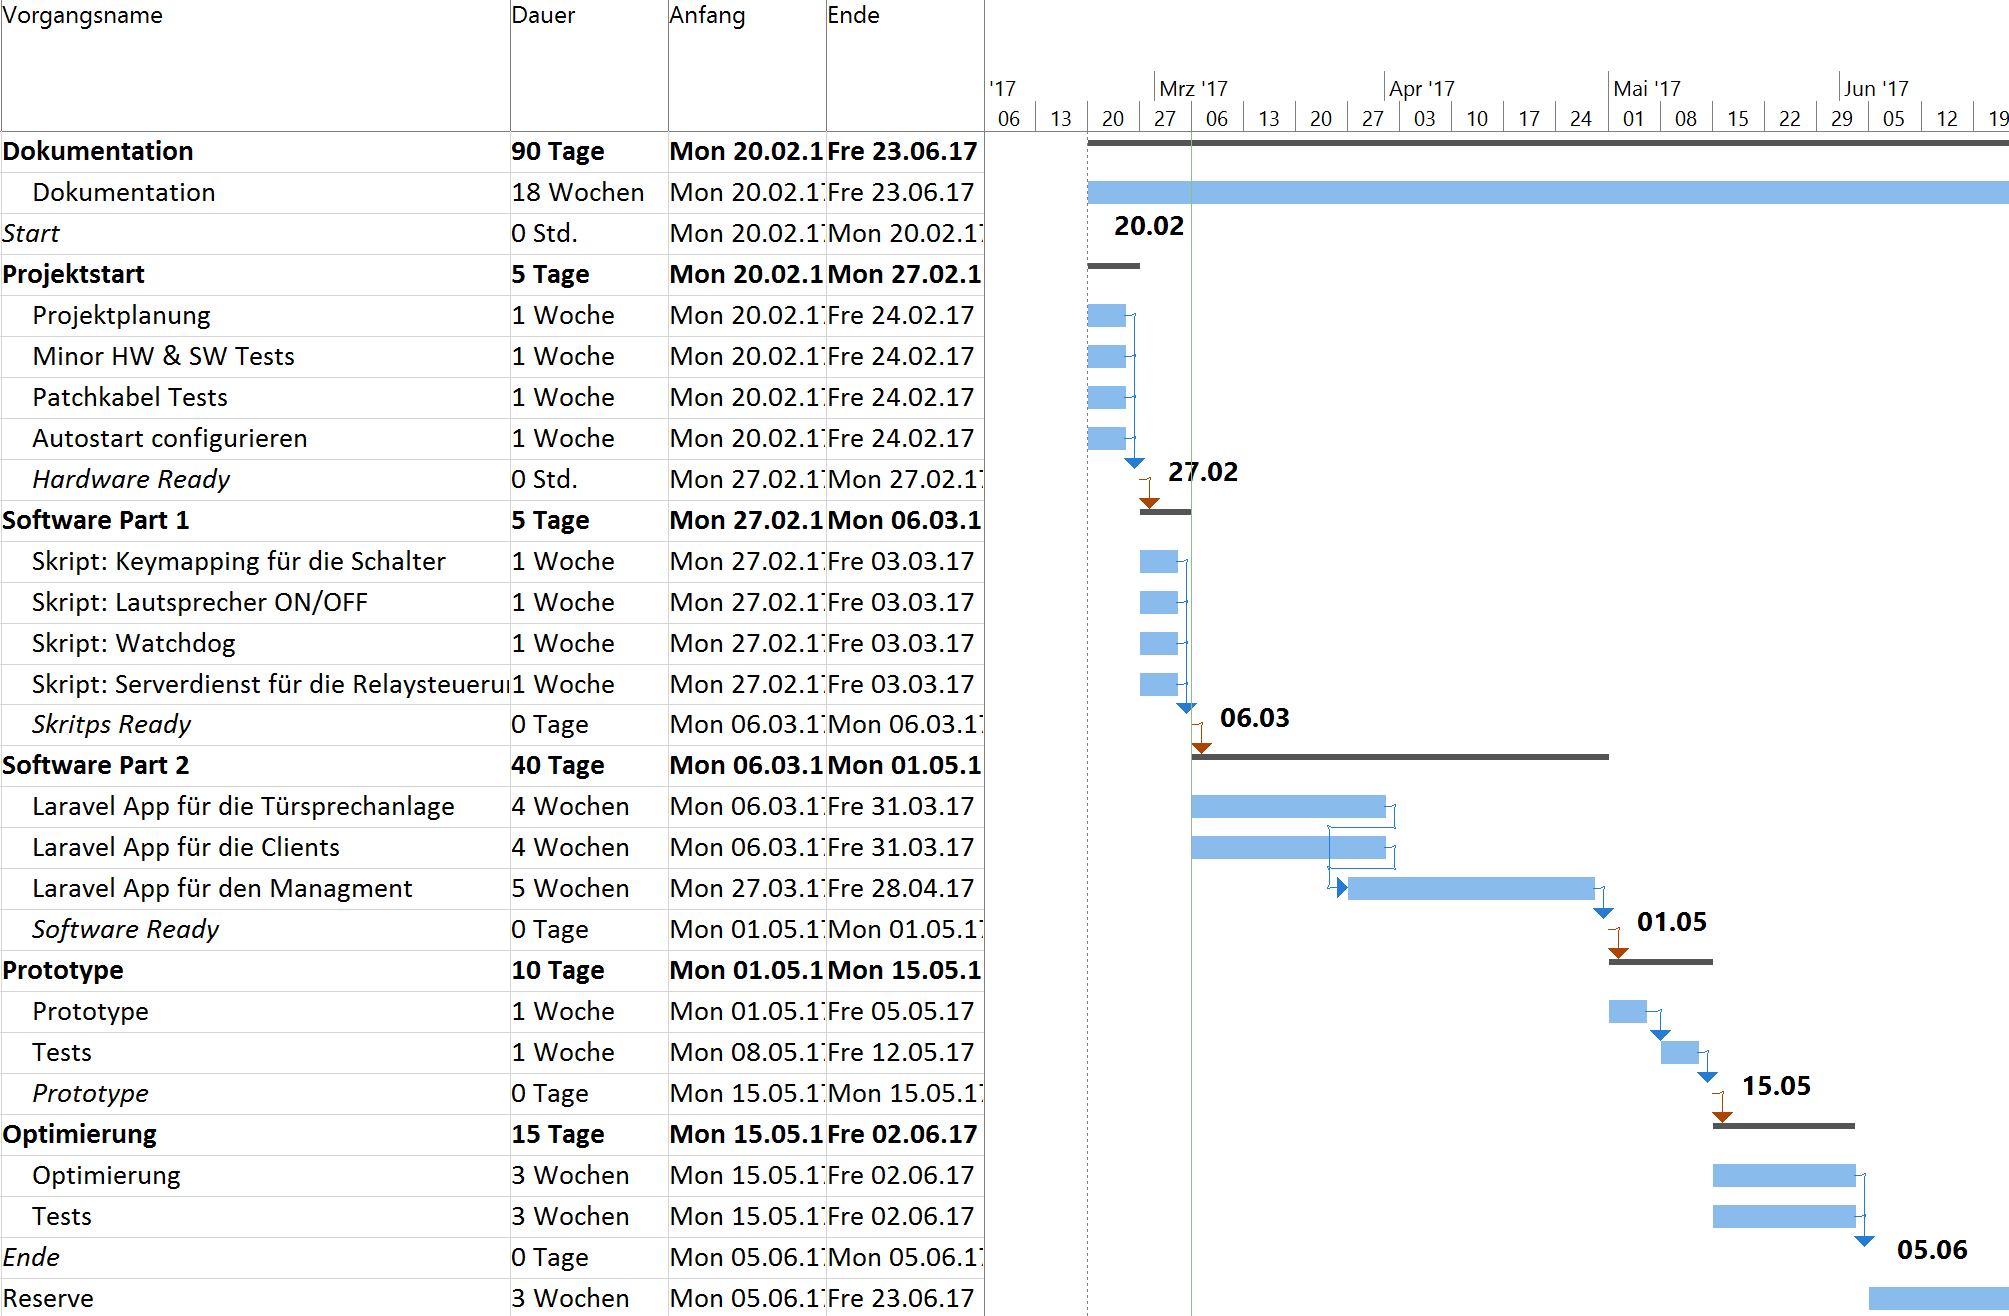
\includegraphics[width=0.9\textwidth]{projektPlanung}
		\caption[Projektplanung]{Projektplanung}
		\label{fig:projektPlanung}
	\end{center}
\end{figure}


\newpage
